% REMEMBER: You must not plagiarise anything in your report. Be extremely careful.
\documentclass{l4proj}

%==============================================================================
% Put any additional packages here
% You can add any packages you want, as long as it does not alter the overall format (e.g. don't change the margins or the reference style).
%
\usepackage{pdfpages} % if you want to include a PDF for an ethics checklist, for example


\begin{document}

%==============================================================================
%% METADATA
\title{Automatic Illustration of Text via Multimodal Interaction}
\author{Stergious Aji (2546916A)}
\date{\today}

\maketitle

%==============================================================================
%% ABSTRACT
\begin{abstract}
    This paper describes a system that automatically illustrates textual information present in audio sources, in addition to a ground truth construction interface for automatic videography generation systems.
    
    Users can use this system as a standard automated videography tool that generates videos with relevant imagery appearing in time with the text in the audio. Alternatively, they can build ground truth data for various audio sources. This ground truth would consist of timing information as well as sets of true labelled images for each chunk within the audio.

    
    
    % Every abstract follows a similar pattern. Motivate; set aims; describe work; explain results.
    % \vskip 0.5em
    % ``XYZ is bad. This project investigated ABC to determine if it was better. 
    % ABC used XXX and YYY to implement ZZZ. This is particularly interesting as XXX and YYY have
    % never been used together. It was found that  
    % ABC was 20\% better than XYZ, though it caused rabies in half of subjects.''
\end{abstract}

%==============================================================================
%% ACKNOWLEDGEMENTS
% \chapter*{Acknowledgements}
% Enter any acknowledgements here. This is optional; you may leave this blank if you wish, or remove the entire chapter
%
% We give thanks to the Gods of LaTeX, who in their eternal graciousness, have granted that this document may compile without errors or overfull hboxes.

%==============================================================================
% EDUCATION REUSE CONSENT FORM
% If you consent to your project being shown to future students for educational purposes then insert your name and the date below to  sign the education use form that appears in the front of the document. You must explicitly give consent if you wish to do so.
% If you sign, your project may be included in the Hall of Fame if it scores particularly highly.
%
% Please note that you are under no obligation to sign this declaration, but doing so would help future students.

\def\consentname {Stergious Aji} % your full name
\def\consentdate {\today} % the date you agree
\educationalconsent


%==============================================================================
\tableofcontents
%==============================================================================
%% Notes on formatting
%==============================================================================
% The first page, abstract and table of contents are numbered using Roman numerals and are not included in the page count. 
%
% From now on pages are numbered using Arabic numerals. Therefore, immediately after the first call to \chapter we need the call \pagenumbering{arabic} and this should be called once only in the document. 
%
%
% The first Chapter should then be on page 1. 

% PAGE LIMITS
% You are allowed 40 pages for a 40 credit project and 30 pages for a 20 credit report. This includes everything numbered in Arabic numerals (excluding front matter) up to but *excluding the appendices and bibliography*.
%
% FORMATTING
% You must not alter text size (it is currently 10pt) or alter margins or spacing. Do not alter the bibliography style. 
%
%================================================================================
%
% IMPORTANT
% The chapter headings and structure here are **suggestions**. You don't have to follow this model if it doesn't fit your project. Every project should have an introduction and conclusion, however.  If in doubt, your supervisor can give you specific guidance; their view takes precedence over the structure suggested here.
%
%================================================================================
\chapter{Introduction}
% reset page numbering. Don't remove this!
\pagenumbering{arabic} 

% Why should the reader care about what are you doing and what are you actually doing?
This chapter serves to outline the motivations for creating an automatic videography tool, as well as the rationale for a subsequent interface for annotating ground truths, specifically using multimodal representations of images and text. 

% \textbf{Motivate} first, then state the general problem clearly. 
\section{Motivations}
\subsection{Automatic Videography}
Text-to-image retrieval is a vast topic that has gained increased interest in recent years, contributing to many real-world applications in today's media-heavy landscape. One of the key areas that have expanded, due to  advancements in image retrieval technology, is automated videography. The rise in video production, both in terms of the number of people making video content and the frequency of videos being made daily \citep{rise_video}, has demanded a drive for more automated systems. This is especially true for music which often has no accompanying video content on popular platforms like \cite{youtube}. This can be for a number of reasons, for instance, no official music video has been created by the artist due to a lack of funding or song popularity, or the audio track could be digitised from an older format, like vinyl. 

Furthermore, such a tool is not restricted to just music tracks. It can be useful for illustrating educational content and podcasts. This would not only increase the accessibility of the subject but, studies have shown that users take in more information from multimodal content compared to text-only or audio-only content \citep{benefits_of_mmv}. Increased engagement means an improved learning experience as a video can encompass three different modes of the same information simultaneously including, visual, audial, and textual. This makes it more suited for people of different learning lifestyles present in Fleming's VARK acronym \citep{vark}.

One of the main motivations for this project is to improve and add on to a previous project, the Automatic Videography of Audio Tracks of Songs by \cite{parker}. This thesis achieved a working automated videography tool, focused on audio tracks sourced from YouTube, however, it suffered from a number of drawbacks that we aim to resolve with this project. A more in-depth review of the thesis is conducted in the Background Section \ref{sec:background_parker}.

\subsection{Ground-Truth Annotation Interface}
With an evergrowing supply of automatic videography systems, it is important to perform evaluations and compare their relevant performances in completing set tasks. However, we found that, currently, there is a lack of objective procedures for evaluating comparative performances between different systems. More specifically in measuring their accuracy at image retrieval from text. Image relevance can and has been assessed with qualitative user surveys but this can often be very subjective on personal preferences and present moods. More importantly, to evaluate a new system, more user studies must be conducted with the same demographic of people if the goal is to compare against the results of a previously evaluated system. This is impractical, not to mention, time-consuming, and ultimately producing unrepeatable and biased evaluations.

This can be mitigated, if instead, a set of true labels are annotated beforehand for provided audio sources which can then be used to evaluate any number of videography systems on those same audio sources. It is vital that a static image collection is used for ground truth constructing and evaluating in order to produce repeatable and standardised performance metrics.

This called for a user-friendly interface to assess the relevance of images from the textual content present in the inputted audio source. Under the hood, this ground-truth constructor interface can use the same pipeline as the automated videography system that we are creating. 


\section{Aims}
This project aims to produce a piece of software that can take any audio source and automatically generate a video from it. The video will consist of timely imagery corresponding to the textual content present in the audio. In addition, this software will include a novel annotation interface for assessing image relevance from text prompts. This will let the user construct a set of ground truths for each portion of the given audio source. This will be achieved by letting the annotator select the set of images that they perceive as the most fitting to the accompanying text or song lyric in the given chunk of audio. This set of images will be picked from a top-$k$ which will be retrieved using our system.

Since there is a high priority for precise ground truth construction, the software must be intuitive to use with clear instructions for the user to follow. We must, therefore, aim to produce a user-friendly interface in an easily accessible platform. Additionally, since the aim is for this application to be used by anyone, appropriate error handling must be in place to accommodate users from a wide area of technical backgrounds. We also aim to make our system modular in design. This way, more technical users would be able to swap in any static image collection with minimal configuring if required.

We aim to use the completed annotation interface to produce ground truths for a pre-selected list of audio sources. This data will be made available in an accessible format for a number of different use cases. Firstly, this data can be used to measure the quality of automated videography systems using standard IR metrics (CITE) like Average Precision, F-Measure and the Normalised Discounted Cumulative Gain (nDCG). However, the data will not be restricted to the task of automatic videography, due to it simply consisting of a set of relevance assessments of images from text. Hence, the data can be used in existing or new text-to-image research in general. A recent example of such a possible use case is investigating the effeciveness of Variable Depth Pooling (CITE), more details are discussed in the Background section (REF).

Finally, as stated in our motivations, we wish to fix the limitations of the previous videography generation system by Parker as well as expand upon its functionality. We aim to, generalise the application of the tool to any audio source, not just restrict it to sourcing from YouTube videos. This also means, our tool must be able to support transcription of multiple languages. We aim to tackle the image retrieval process using a different approach that introduces semantics in order to retrieve more relevant images.

In order to justify creating a novel annotation interface, we must first explore existing solutions and their corresponding strengths and limitations.


%================================================================================
\chapter{Background}
This chapter serves to lay the foundations in order to provide the needed context to understand the scope of this project. Firstly, an explorative analysis of the history and origins of the field of text-to-image retrieval will be conducted. This will be followed by a discussion of the recent advancements of contrastive learning multimodal models with vision transformers. A thorough review of the previous thesis on automatic videography will be given in order to fully discern the motivations and aims for this project. Next, an outline of what current solutions exist to solve our problem of annotating images from text queries will be provided. Finally, a literature review on recent research on Variable Depth Pooling will be carried out which aims to provide further insight on the weight of the potential data we can produce using our solution.

\section{The History of Text-to-Image Retrieval}



\section{CLIP}



\section{Automatic Videography of Audio Tracks of Songs}
\label{sec:background_parker}
\subsection{Problems with the Previous Thesis}
In order to elicit what requirements are necessary, we must look at the problems identified in the previous thesis.
The previous Automatic Videography system implemented by Andrew Parker made many achievements in generating complementary videos for audio tracks. However, it was restricted to the YouTube platform and emerged with a number of unforeseen drawbacks. 

Firstly, the metadata from YouTube was found to be unreliable in obtaining the artist's name and the song title of the song. Therefore, this information was acquired from the user inputting the correct details when using the system. This can be problematic since this requires the user to perform more work of researching and correctly typing in this information which is prone to errors. 

The previous system also relied on many different Application Programming Interfaces (APIs) like YAKE (Yet Another Keyword Extractor) \cite{yake}(CITE) for keyword extraction, and Google Images Search \cite{google_images}(CITE) to download the images. This places a high dependency on these APIs which may not be kept maintained or present version collisions with other packages. In fact, the AutoLyrixAlign API \cite{autolyrixalign}(CITE), which was used for Forced Alignment of the transcription with the audio, has been deprecated at the time of writing.

The previous system also suffered from frequent non-relevant images being retrieved. This was because the semantics of the keywords were being ignored when searching through Google Images. Furthermore, because of this, keywords with many meanings in the English language often resulted in the wrong images being retrieved. 

The final problem observed, which directly spawned our idea of ground truth building, was the user evaluations of the final videography system. The user surveys showed a mixed, but generally positive evaluation of the system. However, the highly varying ratings and the answers to the open-ended questions highlighted the extensive time and effort required to conduct qualitative evaluations on automated videography systems which ultimately produced subjective and unrepeatable results. (REWRITE)

Now that we have identified the main [pitfalls] from the previous system, it makes designing the list of requirements for our system a much simpler task.

\subsection{Improvements to the Previous Thesis}
multilingual

work on any audio source

use semantics with multimodal spaces



\section{Similar Technologies}



\section{The Bigger Picture}
Exploring the background of the project through a review of its history and past accomplishments within the field is essential to establish its significance and justify its existence. By looking at existing solutions to the problem and their contrasting approaches provides valuable insight into which direction we take our project. Nevertheless, it is equally important to envisage the potential applications of our project beyond its primary focus of automated videography. For this reason, we look into recent research that aims to reduce relevance assessment effort by employing query-specific variable depth pooling (CITE) and how ground truths constructed using our proposed annotation tool could be beneficial in this research area.

\subsection{Query-specific Variable Depth Pooling}
This paper proposes a novel approach to 'pooling', a common practice in IR evaluation in order to retrieve the top-$k$ relevant items using a range of different retrieval systems from a large collection. It is conventional to set the depth, $k$, to a constant regardless of the specific query. However, the central idea presented in the research is that by adjusting the depth depending on the query, the relevance annotation effort can be minimised. The authors suggest the rationale behind this idea is that some queries may have fewer relevant items in the collection, while others may have a larger number. 
% Therefore, by adapting the depth of the pool to the specific query by estimating its performance, the annotation effort can be reduced considerably.







%================================================================================
\chapter{Analysis/Requirements}
This chapter serves to break down the high-level aims of the project in order to produce a list of functional and non-functional requirements, ordered by priority. This will directly determine the design and implementation of the project.

\section{Requirements Elicitation}
In order to elicit the list of requirements, a number of user scenarios are created. These are imagined scenarios of users that would directly benefit from such an application. This type of requirements gathering, most commonly used in agile software development projects, places the focus on the end-user, rather than the developer. Therefore, this prioritises the features that an end-user requires to fulfill their goals rather than designing the development process around what is easy to implement. Another benefit of this method is that it mitigates the risk of potential flaws at a very early stage. It is much easier to accommodate any flaws before any design or implementation is undertaken rather than finding them out during the evaluation stages with real users. It gets progressively more difficult to change the existing design the further we are down the development process.


\subsection{User Scenarios}
\subsubsection{User Scenario 1: Anna} is a young secondary school teacher who has started recording her classes in response to the recent shift in online learning. She regularly posts her recordings to an online platform supported by the school. However, she has had a few complaints from her students that her recordings are not engaging enough and that it is difficult to see what she writes on the board. Anna strives to provide the best for her students and wishes she could make her recordings more engaging by illustrating the concepts she talks about in her audio recordings. However, she does not know anything about video production and is worried about the time required to learn and edit videos daily. She wishes for a tool that automatically illustrates her audio recordings in a swift manner to produce videos with captions.

\subsubsection{User Scenario 2: William} has recently built two new Automated Videography Generator tools that use differing ranking procedures to retrieve the top images from the text. He has performed some user studies, where he asked a number of users to watch and rate the videos generated by both systems on the same audio tracks. He used A/B testing in order to compare the performances of his two systems. However, the user studies resulted in very mixed results, with some users rating system $A$ highly while others rated system $B$ as better. Furthermore, upon closer inspection, he found that the user ratings varied wildly depending on the audio tracks used. This was problematic since the user studies took over 2 hours to complete and William is unwilling to conduct another when it is unclear if the results would even improve. William wished that he could objectively evaluate his systems against a set of ground truths. He would be able to use this to obtain quantitative metrics for each system that he could compare giving a clear answer to which ranking procedure is better.

\subsubsection{User Scenario 3: Emily} is a software developer who is part of a small team who is building a new Automatic Videography Generator. Her manager has given her the tedious task of creating ground truths for a predetermined set of audio sources from YouTube. This process requires manually annotating images that are the most fitting for the textual content within the audio. This is a very time-consuming process since she must listen to the audio track multiple times in order to accurately transcribe the textual content. Following this, she must manually record the locations of the annotated images in a spreadsheet. Her manager has also assigned a colleague to go double-check each annotation made. She wishes for a tool that automatically transcribes the audio and provides an easy-to-use interface to annotate images that can be edited after the fact. 


\subsection{User Stories}
\begin{itemize}
    \item As a user of the application, I want to upload audio files, so that I can generate a video from it or construct ground truths for it.
    \item As a user of the application, I want to specify YouTube URLs, so that its  extracted audio can be used as the source.
    \item As a user of the application, I want to build and download ground truths, so that I can use them to evaluate my system.
    \item As a user of the application, I want to edit previously made ground truths, so that I can fix any mistakes made.
    \item As a user of the application, I want to view the full audio transcription, so that I can annotate specific audio chunks.
    \item As a user of the application, I want to view and download the generated video, so that I can share it and upload it to any platform.
\end{itemize}


\section{Requirements}
In order to formalise and prioritise the main requirements identified, the MoSCoW method (CITE) was chosen. Due to the restricted nature of this project, it is not feasible to develop every feature to make the most ideal system, therefore, working on features. 
It would be ideal to implement every requirement specified, however, this is not 

EXPLAIN FUNCTIONAL AND NON-FUNCTIONAL REQS

\subsection{Functional Requirements}
\begin{itemize}
    \item \textbf{Must Have:} Ability to upload an audio file as an input audio source.
    \item \textbf{Must Have:} Ability to specify a YouTube video URL as an audio source.
    \item \textbf{Must Have:} Ability to view the full audio transcription.
    \item \textbf{Must Have:} Ability to generate an illustrated video for any audio source.
    \item \textbf{Must Have:} Ability to view the top-$k$ retrieved images for a given audio chunk.
    \item \textbf{Must Have:} Ability to annotate the most-fitting images for a given audio chunk.
    \item \textbf{Must Have:} Ability to view the text present in a given audio chunk.
    \item \textbf{Must Have:} Ability to view the constructed ground truth data.
    \item \textbf{Must Have:} Ability to download the constructed ground truth data in a portable format.
    \item \textbf{Should Have:} Ability to view previously processed audio sources, generated videos and constructed ground truths.
    \item \textbf{Should Have:} Ability to edit previously made ground truths.
    \item \textbf{Should Have:} Ability to support multilingual audio sources.
    \item \textbf{Could Have:} Ability to load ground truths for editing.
    \item \textbf{Could Have:} Ability to view the percentage complete for ground truth construction of processed audio sources.
    \item \textbf{Could Have:} Ability to reconfigure the static image collection location.
    \item \textbf{Could Have:} Ability to save or skip chunks with repeating textual content when ground truth constructing.
\end{itemize}

\subsection{Non-Functional Requirements}
\begin{itemize}
    \item \textbf{Should Have:} The application being accessible using any Operating System platform.
    \item \textbf{Should Have:} The application having a presentable user interface that is easy-to-use for any user.
    \item \textbf{Should Have:} The application with appropriate error handling.
    \item \textbf{Should Have:} The application displaying progress bars for long loading times.
    \item \textbf{Should Have:} The application being fast and responsive.
    \item \textbf{Should Have:} The system being able to recognise music tracks to retrieve the artist name and song title.
    \item \textbf{Should Have:} The application being able to provide a transcription for any audio source with relative timestamps.
    \item \textbf{Should Have:} The text-to-image retrieval using semantics in order to retrieve more relevant images.
    \item \textbf{Should Have:} The videos being generated in a reasonable amount of time.
    \item \textbf{Should Have:} The images being of high quality in the generated videos.
    \item \textbf{Could Have:} The application being designed modularly to configure any static image collection.
    \item \textbf{Could Have:} The videos including text as well as images.
    \item \textbf{Could Have:} The application visually differentiating between previously processed audio sources.
    \item \textbf{Could Have:} The system performing tempo or beat analysis to appropriately time image changes.
\end{itemize}

% What is the problem that you want to solve, and how did you arrive at it?
% \section{Guidance}
% Make it clear how you derived the constrained form of your problem via a clear and logical process. 

% The analysis chapter explains the process by which you arrive at a concrete design. In software 
% engineering projects, this will include a statement of the requirement capture process and the
% derived requirements.

% In research projects, it will involve developing a design drawing on
% the work established in the background, and stating how the space of possible projects was
% sensibly narrowed down to what you have done.

%================================================================================
\chapter{Design}
How is this problem to be approached, without reference to specific implementation details? 
\section{Guidance}
Design should cover the abstract design in such a way that someone else might be able to do what you did, 
but with a different language or library or tool. This might include overall system architecture diagrams,
user interface designs (wireframes/personas/etc.), protocol specifications, algorithms, data set design choices,
among others. Specific languages, technical choices, libraries and such like should not usually appear in the design. These are implementation details.


%================================================================================
\chapter{Implementation}
What did you do to implement this idea, and what technical achievements did you make?
\section{Guidance}
You can't talk about everything. Cover the high level first, then cover important, relevant or impressive details.

\section{General guidance for technical writing}

These points apply to the whole dissertation, not just this chapter.

\subsection{Figures}
\emph{Always} refer to figures included, like Figure \ref{fig:relu}, in the body of the text. Include full, explanatory captions and make sure the figures look good on the page.
You may include multiple figures in one float, as in Figure \ref{fig:synthetic}, using \texttt{subcaption}, which is enabled in the template.


% Figures are important. Use them well.
\begin{figure}[htb]
    \centering
    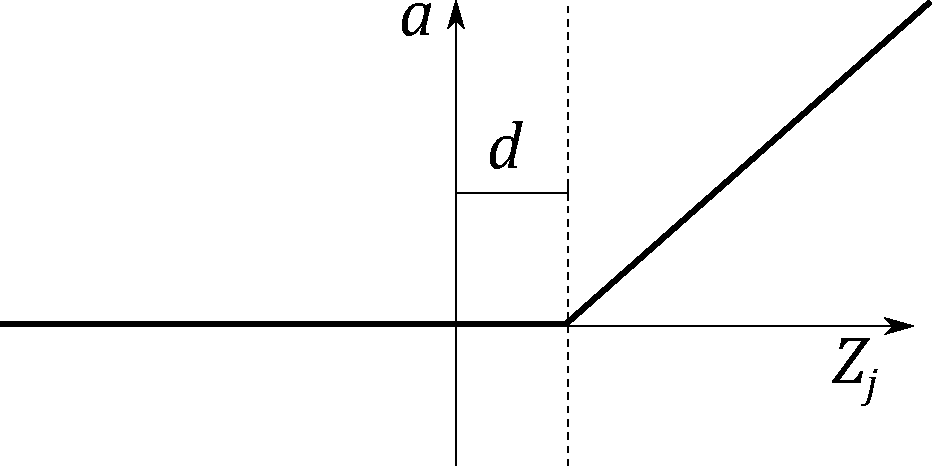
\includegraphics[width=0.5\linewidth]{images/relu.pdf}    

    \caption{In figure captions, explain what the reader is looking at: ``A schematic of the rectifying linear unit, where $a$ is the output amplitude,
    $d$ is a configurable dead-zone, and $Z_j$ is the input signal'', as well as why the reader is looking at this: 
    ``It is notable that there is no activation \emph{at all} below 0, which explains our initial results.'' 
    \textbf{Use vector image formats (.pdf) where possible}. Size figures appropriately, and do not make them over-large or too small to read.
    }

    % use the notation fig:name to cross reference a figure
    \label{fig:relu} 
\end{figure}


\begin{figure}[htb] 
    \centering
    \begin{subfigure}[b]{0.45\textwidth}
        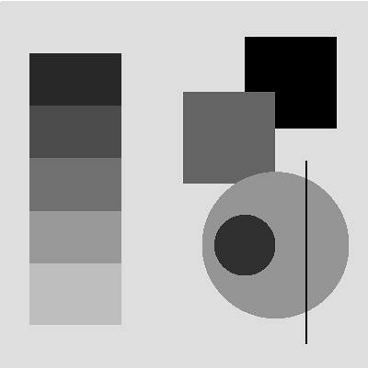
\includegraphics[width=\textwidth]{images/synthetic.png}
        \caption{Synthetic image, black on white.}
        \label{fig:syn1}
    \end{subfigure}
    ~ %add desired spacing between images, e. g. ~, \quad, \qquad, \hfill etc. 
      %(or a blank line to force the subfigure onto a new line)
    \begin{subfigure}[b]{0.45\textwidth}
        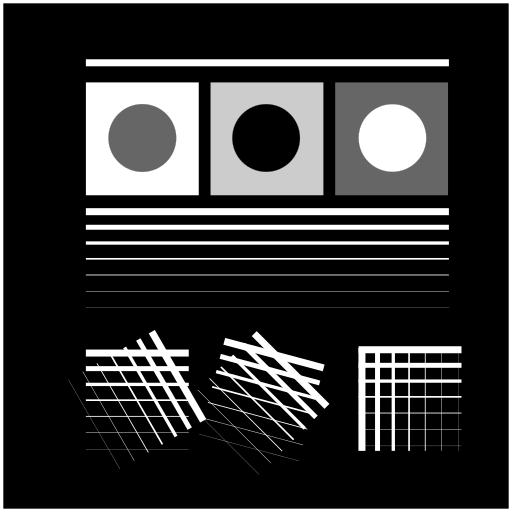
\includegraphics[width=\textwidth]{images/synthetic_2.png}
        \caption{Synthetic image, white on black.}
        \label{fig:syn2}
    \end{subfigure}
    ~ %add desired spacing between images, e. g. ~, \quad, \qquad, \hfill etc. 
    %(or a blank line to force the subfigure onto a new line)    
    \caption{Synthetic test images for edge detection algorithms. \subref{fig:syn1} shows various gray levels that require an adaptive algorithm. \subref{fig:syn2}
    shows more challenging edge detection tests that have crossing lines. Fusing these into full segments typically requires algorithms like the Hough transform.
    This is an example of using subfigures, with \texttt{subref}s in the caption.
    }\label{fig:synthetic}
\end{figure}

\clearpage

\subsection{Equations}

Equations should be typeset correctly and precisely. Make sure you get parenthesis sizing correct, and punctuate equations correctly 
(the comma is important and goes \textit{inside} the equation block). Explain any symbols used clearly if not defined earlier. 

For example, we might define:
\begin{equation}
    \hat{f}(\xi) = \frac{1}{2}\left[ \int_{-\infty}^{\infty} f(x) e^{2\pi i x \xi} \right],
\end{equation}    
where $\hat{f}(\xi)$ is the Fourier transform of the time domain signal $f(x)$.

\subsection{Algorithms}
Algorithms can be set using \texttt{algorithm2e}, as in Algorithm \ref{alg:metropolis}.

% NOTE: line ends are denoted by \; in algorithm2e
\begin{algorithm}
    \DontPrintSemicolon
    \KwData{$f_X(x)$, a probability density function returing the density at $x$.\; $\sigma$ a standard deviation specifying the spread of the proposal distribution.\;
    $x_0$, an initial starting condition.}
    \KwResult{$s=[x_1, x_2, \dots, x_n]$, $n$ samples approximately drawn from a distribution with PDF $f_X(x)$.}
    \Begin{
        $s \longleftarrow []$\;
        $p \longleftarrow f_X(x)$\;
        $i \longleftarrow 0$\;
        \While{$i < n$}
        {
            $x^\prime \longleftarrow \mathcal{N}(x, \sigma^2)$\;
            $p^\prime \longleftarrow f_X(x^\prime)$\;
            $a \longleftarrow \frac{p^\prime}{p}$\;
            $r \longleftarrow U(0,1)$\;
            \If{$r<a$}
            {
                $x \longleftarrow x^\prime$\;
                $p \longleftarrow f_X(x)$\;
                $i \longleftarrow i+1$\;
                append $x$ to $s$\;
            }
        }
    }
    
\caption{The Metropolis-Hastings MCMC algorithm for drawing samples from arbitrary probability distributions, 
specialised for normal proposal distributions $q(x^\prime|x) = \mathcal{N}(x, \sigma^2)$. The symmetry of the normal distribution means the acceptance rule takes the simplified form.}\label{alg:metropolis}
\end{algorithm}

\subsection{Tables}

If you need to include tables, like Table \ref{tab:operators}, use a tool like https://www.tablesgenerator.com/ to generate the table as it is
extremely tedious otherwise. 

\begin{table}[]
    \caption{The standard table of operators in Python, along with their functional equivalents from the \texttt{operator} package. Note that table
    captions go above the table, not below. Do not add additional rules/lines to tables. }\label{tab:operators}
    %\tt 
    \rowcolors{2}{}{gray!3}
    \begin{tabular}{@{}lll@{}}
    %\toprule
    \textbf{Operation}    & \textbf{Syntax}                & \textbf{Function}                            \\ %\midrule % optional rule for header
    Addition              & \texttt{a + b}                          & \texttt{add(a, b)}                                    \\
    Concatenation         & \texttt{seq1 + seq2}                    & \texttt{concat(seq1, seq2)}                           \\
    Containment Test      & \texttt{obj in seq}                     & \texttt{contains(seq, obj)}                           \\
    Division              & \texttt{a / b}                          & \texttt{div(a, b) }  \\
    Division              & \texttt{a / b}                          & \texttt{truediv(a, b) } \\
    Division              & \texttt{a // b}                         & \texttt{floordiv(a, b)}                               \\
    Bitwise And           & \texttt{a \& b}                         & \texttt{and\_(a, b)}                                  \\
    Bitwise Exclusive Or  & \texttt{a \textasciicircum b}           & \texttt{xor(a, b)}                                    \\
    Bitwise Inversion     & \texttt{$\sim$a}                        & \texttt{invert(a)}                                    \\
    Bitwise Or            & \texttt{a | b}                          & \texttt{or\_(a, b)}                                   \\
    Exponentiation        & \texttt{a ** b}                         & \texttt{pow(a, b)}                                    \\
    Identity              & \texttt{a is b}                         & \texttt{is\_(a, b)}                                   \\
    Identity              & \texttt{a is not b}                     & \texttt{is\_not(a, b)}                                \\
    Indexed Assignment    & \texttt{obj{[}k{]} = v}                 & \texttt{setitem(obj, k, v)}                           \\
    Indexed Deletion      & \texttt{del obj{[}k{]}}                 & \texttt{delitem(obj, k)}                              \\
    Indexing              & \texttt{obj{[}k{]}}                     & \texttt{getitem(obj, k)}                              \\
    Left Shift            & \texttt{a \textless{}\textless b}       & \texttt{lshift(a, b)}                                 \\
    Modulo                & \texttt{a \% b}                         & \texttt{mod(a, b)}                                    \\
    Multiplication        & \texttt{a * b}                          & \texttt{mul(a, b)}                                    \\
    Negation (Arithmetic) & \texttt{- a}                            & \texttt{neg(a)}                                       \\
    Negation (Logical)    & \texttt{not a}                          & \texttt{not\_(a)}                                     \\
    Positive              & \texttt{+ a}                            & \texttt{pos(a)}                                       \\
    Right Shift           & \texttt{a \textgreater{}\textgreater b} & \texttt{rshift(a, b)}                                 \\
    Sequence Repetition   & \texttt{seq * i}                        & \texttt{repeat(seq, i)}                               \\
    Slice Assignment      & \texttt{seq{[}i:j{]} = values}          & \texttt{setitem(seq, slice(i, j), values)}            \\
    Slice Deletion        & \texttt{del seq{[}i:j{]}}               & \texttt{delitem(seq, slice(i, j))}                    \\
    Slicing               & \texttt{seq{[}i:j{]}}                   & \texttt{getitem(seq, slice(i, j))}                    \\
    String Formatting     & \texttt{s \% obj}                       & \texttt{mod(s, obj)}                                  \\
    Subtraction           & \texttt{a - b}                          & \texttt{sub(a, b)}                                    \\
    Truth Test            & \texttt{obj}                            & \texttt{truth(obj)}                                   \\
    Ordering              & \texttt{a \textless b}                  & \texttt{lt(a, b)}                                     \\
    Ordering              & \texttt{a \textless{}= b}               & \texttt{le(a, b)}                                     \\
    % \bottomrule
    \end{tabular}
    \end{table}
\subsection{Code}

Avoid putting large blocks of code in the report (more than a page in one block, for example). Use syntax highlighting if possible, as in Listing \ref{lst:callahan}.

\begin{lstlisting}[language=python, float, caption={The algorithm for packing the $3\times 3$ outer-totalistic binary CA successor rule into a 
    $16\times 16\times 16\times 16$ 4 bit lookup table, running an equivalent, notionally 16-state $2\times 2$ CA.}, label=lst:callahan]
    def create_callahan_table(rule="b3s23"):
        """Generate the lookup table for the cells."""        
        s_table = np.zeros((16, 16, 16, 16), dtype=np.uint8)
        birth, survive = parse_rule(rule)

        # generate all 16 bit strings
        for iv in range(65536):
            bv = [(iv >> z) & 1 for z in range(16)]
            a, b, c, d, e, f, g, h, i, j, k, l, m, n, o, p = bv

            # compute next state of the inner 2x2
            nw = apply_rule(f, a, b, c, e, g, i, j, k)
            ne = apply_rule(g, b, c, d, f, h, j, k, l)
            sw = apply_rule(j, e, f, g, i, k, m, n, o)
            se = apply_rule(k, f, g, h, j, l, n, o, p)

            # compute the index of this 4x4
            nw_code = a | (b << 1) | (e << 2) | (f << 3)
            ne_code = c | (d << 1) | (g << 2) | (h << 3)
            sw_code = i | (j << 1) | (m << 2) | (n << 3)
            se_code = k | (l << 1) | (o << 2) | (p << 3)

            # compute the state for the 2x2
            next_code = nw | (ne << 1) | (sw << 2) | (se << 3)

            # get the 4x4 index, and write into the table
            s_table[nw_code, ne_code, sw_code, se_code] = next_code

        return s_table

\end{lstlisting}

%==================================================================================================================================
\chapter{Evaluation} 
How good is your solution? How well did you solve the general problem, and what evidence do you have to support that?

\section{Guidance}
\begin{itemize}
    \item
        Ask specific questions that address the general problem.
    \item
        Answer them with precise evidence (graphs, numbers, statistical
        analysis, qualitative analysis).
    \item
        Be fair and be scientific.
    \item
        The key thing is to show that you know how to evaluate your work, not
        that your work is the most amazing product ever.
\end{itemize}

\section{Evidence}
Make sure you present your evidence well. Use appropriate visualisations, 
reporting techniques and statistical analysis, as appropriate. The point is not
to dump all the data you have but to present an argument well supported by evidence gathered.

If you use numerical evidence, specify reasonable numbers of significant digits; don't state ``18.41141\% of users were successful'' if you only had 20 users. If you average \textit{anything}, present both a measure of central tendency (e.g. mean, median) \textit{and} a measure of spread (e.g. standard deviation, min/max, interquartile range).

You can use \texttt{siunitx} to define units, space numbers neatly, and set the precision for the whole LaTeX document. 

% setup siunitx to have two decimal places
\sisetup{
	round-mode = places,
	round-precision = 2
}

For example, these numbers will appear with two decimal places: \num{3.141592}, \num{2.71828}, and this one will appear with reasonable spacing \num{1000000}.



If you use statistical procedures, make sure you understand the process you are using,
and that you check the required assumptions hold in your case. 

If you visualise, follow the basic rules, as illustrated in Figure \ref{fig:boxplot}:
\begin{itemize}
\item Label everything correctly (axis, title, units).
\item Caption thoroughly.
\item Reference in text.
\item \textbf{Include appropriate display of uncertainty (e.g. error bars, Box plot)}
\item Minimize clutter.
\end{itemize}

See the file \texttt{guide\_to\_visualising.pdf} for further information and guidance.

\begin{figure}[htb]
    \centering
    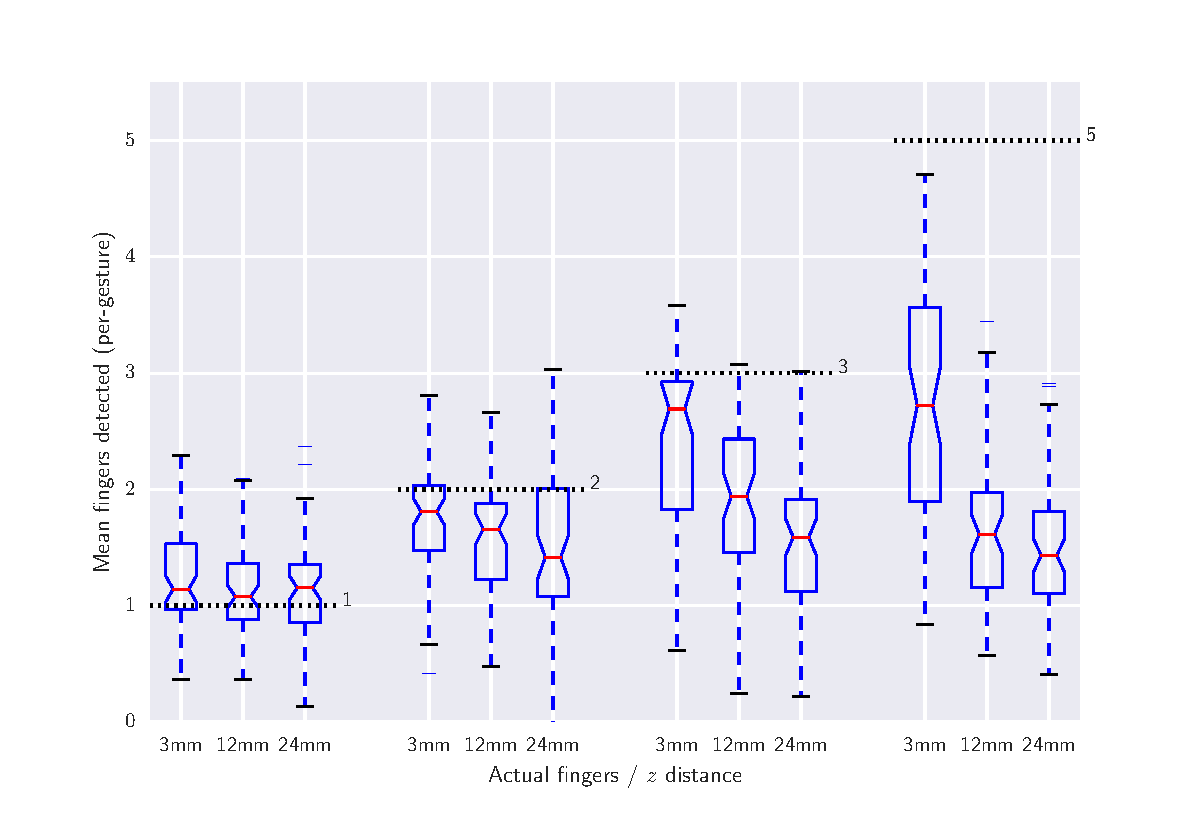
\includegraphics[width=1.0\linewidth]{images/boxplot_finger_distance.pdf}    

    \caption{Average number of fingers detected by the touch sensor at different heights above the surface, averaged over all gestures. Dashed lines indicate
    the true number of fingers present. The Box plots include bootstrapped uncertainty notches for the median. It is clear that the device is biased toward 
    undercounting fingers, particularly at higher $z$ distances.
    }

    % use the notation fig:name to cross reference a figure
    \label{fig:boxplot} 
\end{figure}


%==================================================================================================================================
\chapter{Conclusion}    
Summarise the whole project for a lazy reader who didn't read the rest (e.g. a prize-awarding committee). This chapter should be short in most dissertations; maybe one to three pages.
\section{Guidance}
\begin{itemize}
    \item
        Summarise briefly and fairly.
    \item
        You should be addressing the general problem you introduced in the
        Introduction.        
    \item
        Include summary of concrete results (``the new compiler ran 2x
        faster'')
    \item
        Indicate what future work could be done, but remember: \textbf{you
        won't get credit for things you haven't done}.
\end{itemize}

\section{Summary}
Summarise what you did; answer the general questions you asked in the introduction. What did you achieve? Briefly describe what was built and summarise the evaluation results.

\section{Reflection}
Discuss what went well and what didn't and how you would do things differently if you did this project again.

\section{Future work}
Discuss what you would do if you could take this further -- where would the interesting directions to go next be? (e.g. you got another year to work on it, or you started a company to work on this, or you pursued a PhD on this topic)

%==================================================================================================================================
%
% 
%==================================================================================================================================
%  APPENDICES  

\begin{appendices}

\chapter{Appendices}
 (ETHICS CHECKLIST + INTRODUCTION BRIEF)
 
Use separate appendix chapters for groups of ancillary material that support your dissertation. 
Typical inclusions in the appendices are:

\begin{itemize}
\item
  Copies of ethics approvals (you must include these if you needed to get them)
\item
  Copies of questionnaires etc. used to gather data from subjects. Don't include
  voluminous data logs; instead submit these electronically alongside your source code.
\item
  Extensive tables or figures that are too bulky to fit in the main body of
  the report, particularly ones that are repetitive and summarised in the body.
\item Outline of the source code (e.g. directory structure), 
    or other architecture documentation like class diagrams.
\item User manuals, and any guides to starting/running the software. 
Your equivalent of \texttt{readme.md} should be included.

\end{itemize}

\textbf{Don't include your source code in the appendices}. It will be
submitted separately.



\end{appendices}

%==================================================================================================================================
%   BIBLIOGRAPHY   

% The bibliography style is agsm (Harvard)
% The bibliography always appears last, after the appendices.

\bibliographystyle{agsm}

% Force the bibliography not to be numbered
\renewcommand{\thechapter}{0} 
\bibliography{l4proj}

\end{document}
